\chapter{Domain of Maximal Attraction Verification}
\label{ap:theoremVer}

In this section we are going to verify numerically the Theorem for the Truncated Normal Distribution using Python. For that, we first need to define the generalized normal distribution:

\begin{equation} \label{eq:Normal_PDF}
\phi (x; \mu, \sigma^2) = \frac{1}{\sigma \sqrt{2 \pi}} e^{-\frac{\left( x - \mu \right)^2}{2\sigma^2}}
\end{equation}

\begin{equation} \label{eq:Normal_CDF}
\Phi (x; \mu, \sigma^2) = \int_{-\infty} ^x \phi (t;\mu,\sigma^2) dt
\end{equation}

In Python:

Now, we define the truncated normal distribution in $(0,1)$, because we have a distribution of probabilities:

\begin{equation} \label{eq:TNormal_PDF}
\psi (x; \mu, \sigma^2,0,1) = 
\begin{cases}
0 & \text{ if } x \leq 0 \\
\frac{\phi(x;\mu, \sigma^2)}{\Phi (1; \mu, \sigma^2)-\Phi (0; \mu, \sigma^2)} & \text{ if } 0 < x < 1 \\
0 & \text{ if } x \geq 1
\end{cases}
\end{equation}

\begin{equation} \label{eq:TNormal_CDF}
\Psi (x; \mu, \sigma^2,0,1) = \int_{0} ^x \psi (t;\mu,\sigma^2,0,1) dt
\end{equation}

In Python:

Now, part $(c)$ of the theorem states that sufficient conditions for $\Psi$ to belong to $D(G_3)$, where $G_3$ is the Gumbel distribution are:

\begin{itemize}
\item If $\psi(x) >0$ and is differentiable for all $x$ in $(x_1,\epsilon_1)$ for some $x_1$, and
\begin{equation} \label{eq:partC_theorem}
\lim_{x \rightarrow \epsilon_1} \frac{d}{dx} \left[ \frac{1-\Psi(x)}{\psi(x)} \right] = 0
\end{equation}
\end{itemize}

Numerically, we take arbitrary values for $\mu$ and $\sigma$, then we substitute values for $x$ within our domain $(0,1)$ to obtain the following results.

\begin{figure}[htbp!]
\centering
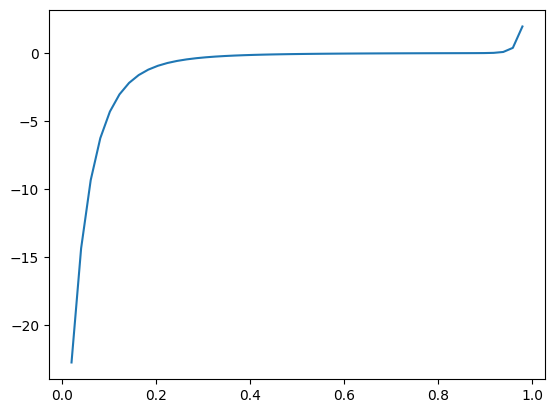
\includegraphics[width=0.7\textwidth]{images/th1052_gumbel_verify.png}
\label{fig:gumbel_verify}
\end{figure}

Note that the function inside the limit on Equation \ref{eq:partC_theorem} tends to $0$ inside the $(0,1)$ interval. Hence, Gumbel distribution can be used as a limiting distribution.